\documentclass{book}
\title{A Computational Tour of Important Problems and Objects of Number Theory}
\author{Math 581f Participants}

\usepackage{amsmath}

\DeclareMathOperator{\Li}{Li}

\usepackage{listings}
\lstdefinelanguage{Sage}[]{Python}
{morekeywords={True,False,sage,singular},
sensitive=true}
\lstset{
  showtabs=False,
  showspaces=False,
  showstringspaces=False,
  commentstyle={\ttfamily\color{dredcolor}},
  keywordstyle={\ttfamily\color{dbluecolor}\bfseries},
  stringstyle ={\ttfamily\color{dgraycolor}\bfseries},
  language = Sage,
  basicstyle={\scriptsize \ttfamily},
  aboveskip=1em,
  belowskip=1em,
  backgroundcolor=\color{lightyellow},
  frame=single
}

\usepackage{color}


\definecolor{lightyellow}{rgb}{1,1,.86}
\definecolor{dblackcolor}{rgb}{0.0,0.0,0.0}
\definecolor{dbluecolor}{rgb}{.01,.02,0.7}
\definecolor{dredcolor}{rgb}{0.8,0,0}
\definecolor{dgraycolor}{rgb}{0.30,0.3,0.30}
\definecolor{graycolor}{rgb}{0.35,0.35,0.35}

\usepackage{graphicx}



\begin{document}
\maketitle
\tableofcontents

\chapter{Introduction}
In this book, we will explore several important central problems and
objects of number theory, and for each to explain how---in practice
(not just theory)---to {\em compute} with them.    Books,
papers, and web sites such as Wikipedia and Mathoverflow often
give excellent descriptions
of mathematical objects, algorithms, data, conjectures, and theorems.
However, they rarely give concrete instructions
so that you can manipulate them on a computer, with enough theoretical
discussion so that you understand the limitations and capabilities of
your tools.  That is the mission of the book you are looking at.


\section{A Tour of the main questions}

The prime numbers $2,3,5,7,11,\ldots, $ have fascinated
mathematicians for thousands of years.  Euclid proved there
are infinitely many: if $p_1,\ldots, p_n$ are primes,
then $p_1\cdots p_n + 1$ is an integer divisible by some
prime $p$ that isn't equal to any $p_i$.

Let's compute the primes up to 100:
\begin{lstlisting}
sage: prime_range(100)
[2, 3, 5, 7, 11, 13, 17, 19, 23, 29, 31, 37, 41, 43, 47, 53, 59, 61, 67, 71,
 73, 79, 83, 89, 97]
\end{lstlisting}
And draw a plot of the function $\pi(x)$ that counts the number of primes up to $x$ for $x<100$.
\begin{center}
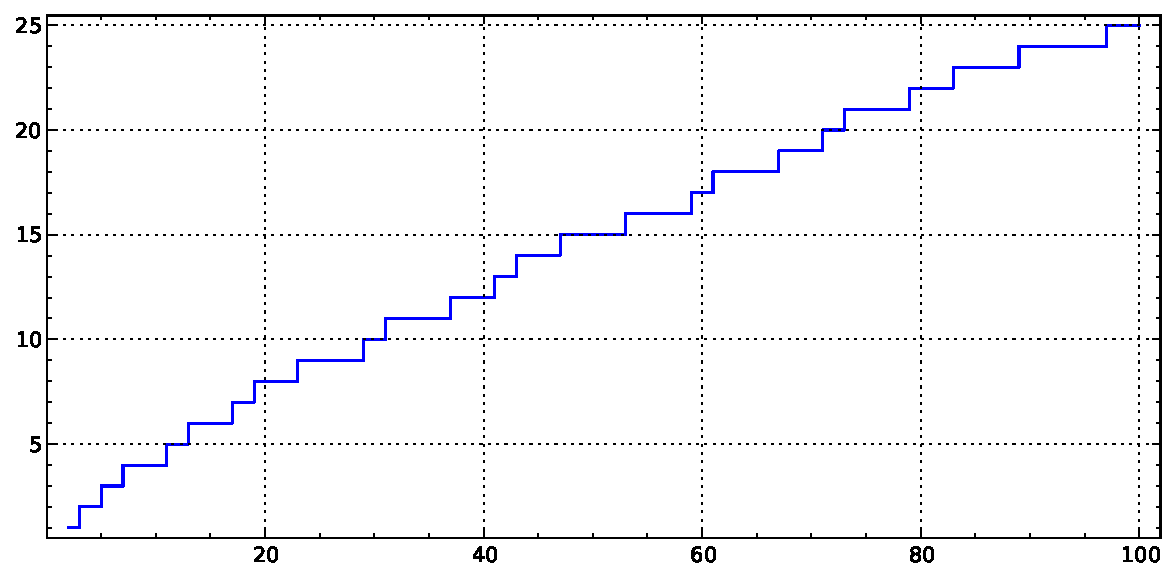
\includegraphics[width=.7\textwidth]{pics/prime_pi-2-100.pdf}
\end{center}

The {\em Prime Number Theorem}, which was proved over a century ago, asserts that $\pi(x) \sim x/\log(x)$:

\begin{lstlisting}
@interact
def f(B=[10^n for n in [2..9]]):
    show(plot(lambda x: prime_pi(x)/(x/log(x)), (x,2,B))
       + line([(0,1),(B,1)],color='red'))
\end{lstlisting}

\begin{center}
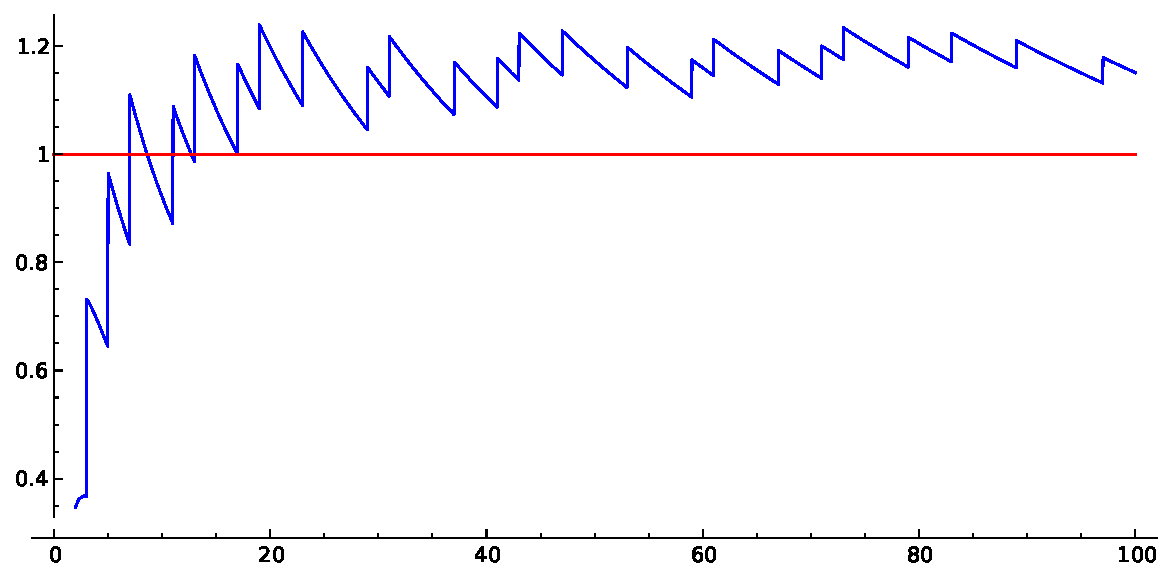
\includegraphics[width=.3\textwidth]{pics/pnt100.pdf}
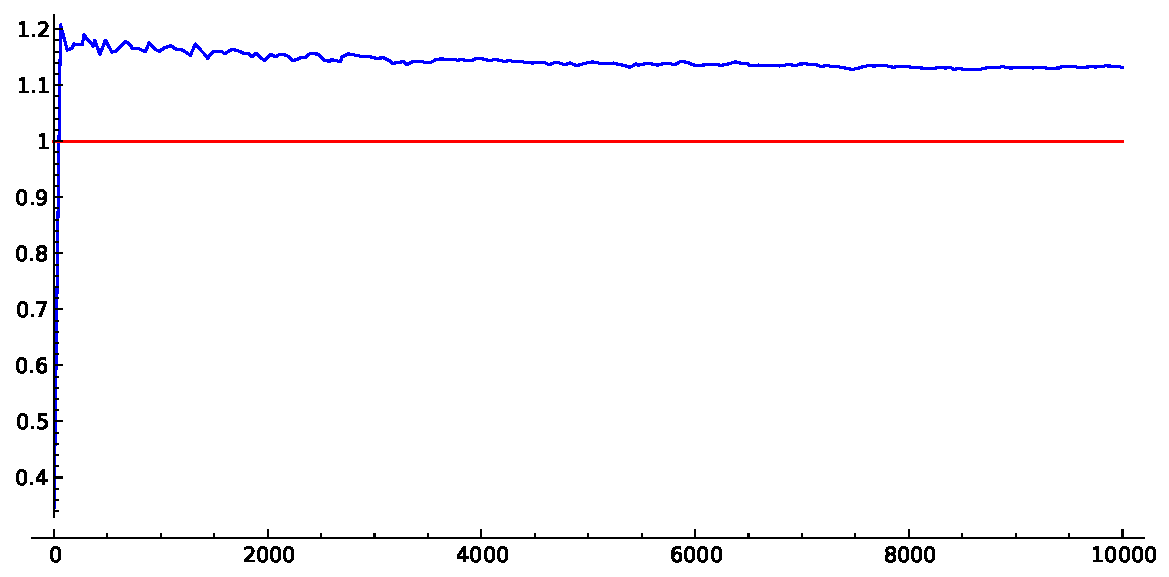
\includegraphics[width=.3\textwidth]{pics/pnt10000.pdf}
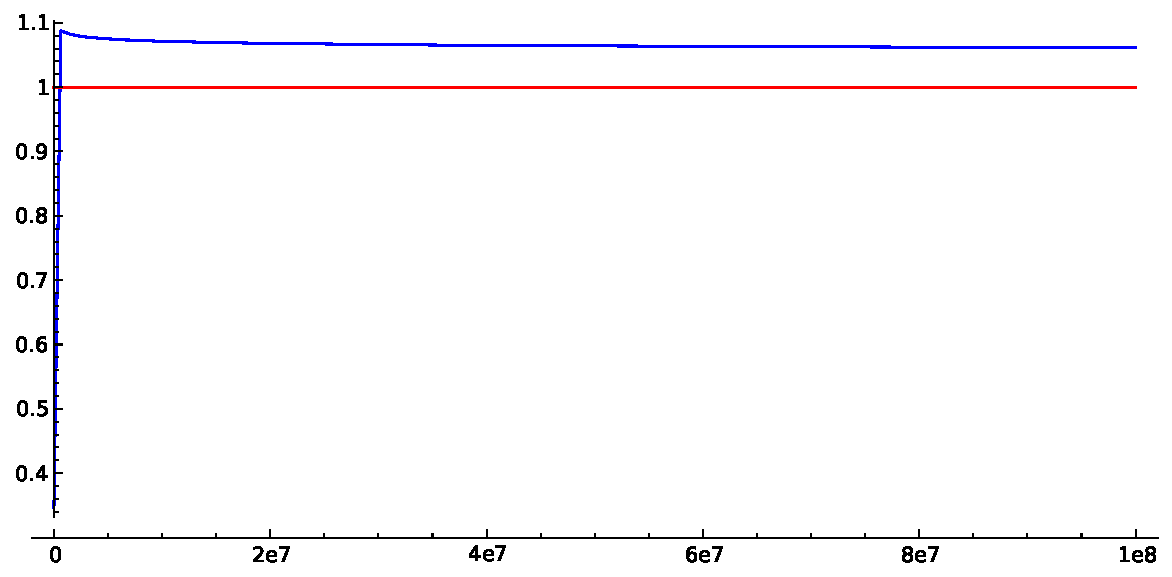
\includegraphics[width=.3\textwidth]{pics/pnt100000000.pdf}
\end{center}

The {\em Riemann Hypothesis}, which remains completely unsolved today,
asserts that for all $x\geq 2.01$,
$$
 |\pi(x) - \Li(x)| \leq \sqrt{x}\cdot \log(x),
$$
where
$$
 \Li(x) = \int_{2}^x \frac{dt}{\log(t)}
$$


\chapter{Prime Numbers}

Main unsolved problem: the Riemann Hypothesis



\section{Infinitely many primes}
\section{The Prime number theorem}
\section{The Riemann hypothesis}
\section{The Explicit Formula}
\section{Generalizations to number fields}


\chapter{Arithmetic of Number Fields}
Main unsolved problem: class number 1 fields

\section{Class groups}
\section{The Gauss class number problem}
\section{Number fields of class number 1}
 (Cohen-lenstra, Bharghava)



\chapter{Diophantine Equations: Fermat and ABC}
Main unsolved problem: ABC conjecture

\section{Fermat's Last Theorem}
\section{The ABC Conjecture}
\section{Generalized Fermat equations}



\chapter{Elliptic Curves}
Important unsolved problem: the BSD conjecture (computing Mordell-Weil groups)

\section{The Group law}
\section{The Mordell-Weil theorem}
\section{Mazur's classification of torsion subroups}
\section{The $L$-series}
analytic continuation and functional equation (modularity)
\section{The Birch and Swinnerton-Dyer conjecture}
\section{The Hasse bound}
\section{The Explicit Formula}



\chapter{Modular Forms}
Important unsolved problem: modularity of elliptic curves
over totally real fields

\section{Ramanujan bound}
\section{Galois representations attached to modular forms}
\section{Modularity of elliptic curves}




\chapter{Public-key Cryptography}

Important unsolved problem: how difficult is the discrete log problem?

\section{Protocols: Diffie-Hellman, RSA, ElGamal, ...}
\section{Discrete log problem (baby-step, giant-step)}



\end{document}

%sagemathcloud={"zoom_width":140}